\documentclass[12pt]{article}
\usepackage{jacob}
\usepackage[left=1.5in,top=1.5in,bottom=1.5in,right=1.5in]{geometry}
\title{}
\date{}
\author{Jacob H. Nie}
\begin{document}

\section*{Problem 19}

\subsection*{Summary of Approach}
First, I calculate the equation that the exact energy eigenvalues must satisfy.  Then I give a strategy for calculating the form of the exact eigenstates, and I show them graphically for a certain setup.  Then, I calculate an approximate form for the energy eigenvalues for both large $n$ and small $L$.  I do this in two ways: by considering the asymptotic behavior of the exact wavefunction, and by using a WKB approximation.  Lastly, I answer some of the further questions.

Many of the numerical calculations and plotting done in this solution can be found in the attached Mathematica notebook.

\subsection*{Exact Solution}

The Hamiltonian in this problem is 
\[
	H = \frac{P^2}{2m} + V(X),
\] 
where $V(X)$ in the $X$-basis is given by
\[
	V(x) = 
	\begin{cases}
		\infty \qquad & x\geq L \\
		Fx \qquad & 0 < x < L \\
		\infty \qquad & x \leq 0.
	\end{cases}
\] 

First, we solve the time-independent Schrodinger equation for $0 < x < L$ and consider the boundary condition $\psi(0) = \psi(L) = 0$ afterwards.
\begin{align*}
	\left( -\frac{\hbar^2}{2m}\frac{\diff ^2}{\diff x ^2} + Fx \right)\psi(x) &= E\psi(x) \\
	\psi ''(x) &= \frac{2m(Fx-E)}{\hbar^2} \psi(x).
\end{align*}
Let us now make the substitutions $u = x - E/F$ and $k = (2mF/\hbar^2)^{1/2}$.  The differential equation becomes
\begin{equation}
	\psi ''(u) - k^2 u \psi(u) = 0.
\end{equation}
We recognize (1) as the Airy equation.  Its solutions are given by 
\begin{equation}
	\psi(u) = A \ \text{Ai}(k^{2/3}u) + B \ \text{Bi}(k^{2/3}u).
\end{equation}
Taking into account the boundary conditions, we have the system of equations:
\begin{align*}
	A \ \text{Ai}\left[ k^{2/3}\left( -\frac{E}{F} \right) \right] + B \ \text{Bi}\left[ k^{2/3}\left(- \frac{E}{F} \right) \right] &= 0 \\
	A \ \text{Ai}\left[ k^{2/3}\left( L-\frac{E}{F} \right) \right] + B \ \text{Bi}\left[ k^{2/3} \left( L - \frac{E}{F} \right) \right] &= 0.
\end{align*}
Here, let us introduce the shorthand
\begin{align*}
	\alpha &= \frac{k^{2/3}E}{F} = \left( \frac{2m}{\hbar^2 F^2} \right)^{1/3} E \\
	\beta &= k^{2/3} L = \left( \frac{2mF}{\hbar^2} \right)^{1/3} L.
\end{align*}
Note that $\alpha$ can be interpreted as a non-dimensional parameter for $E$, and $\beta$ can be interpreted as a non-dimensional parameter for $L$.  There exists a non-trivial solution to $A$ and $B$ in the previous system of equations only if
\begin{equation}
	\text{det}(\alpha, \beta) \equiv \text{Ai}(-\alpha) \ \text{Bi}(\beta - \alpha) - \text{Ai}(\beta - \alpha)\ \text{Bi}(-\alpha) = 0.
\end{equation}
$\text{det}(\alpha,\beta)$ is shown as a contour plot in Figure 1.  

\begin{figure}[ht]
	\centering
	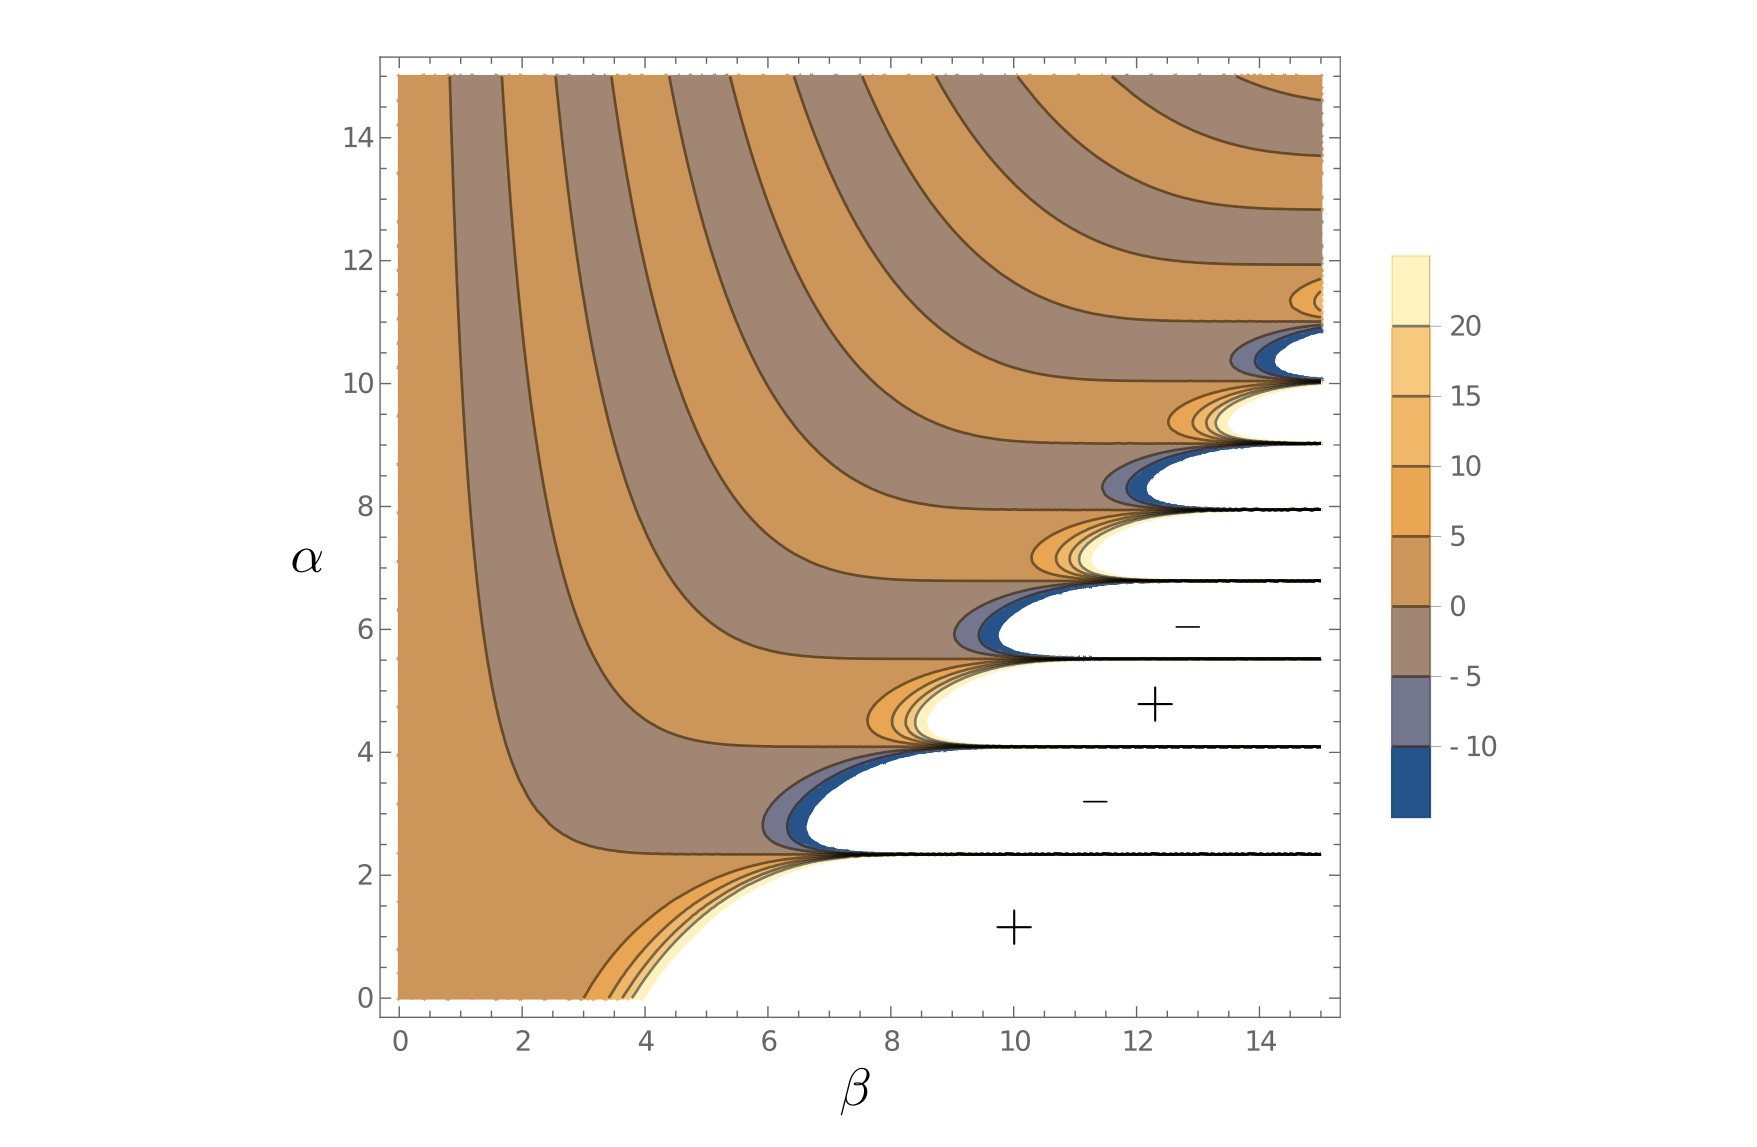
\includegraphics[width=\textwidth]{figures/plot1.png}
	\caption{A contour plot of $\text{det}(\alpha,\beta)$.  $\alpha$ is proportional to the energy eigenvalue and $\beta$ is proportional to the length of the box, so the curves $\text{det}(\alpha,\beta) = 0$ are the plots of the lower energy eigenvalues as a function of box length.}
\end{figure}

To illustrate some of the first few stationary energy eigenfunctions, we select $\beta = 10$.  Then, we solve, numerically, for the first few values of $\alpha$ such that $\text{det}(\alpha, 10) = 0.$  We use these values of $(\alpha,\beta)$ to calculate the values of $A$ and $B$, as defined in the system of equations found above:
\[
	A \ \text{Ai}(-\alpha) + B \ \text{Bi}(-\alpha) = 0.
\]
Then, the un-normalized eigenstates are given by
\[
	\psi(y) = \text{Ai}(y) + \frac{B}{A}\text{Bi}(y),
\] 
on the domain $y \in [\alpha, \beta - \alpha]$.  We plot the first 9 eigenstates in Figure 2.

\begin{figure}[ht]
	\centering
	
\includegraphics[width=\textwidth]{figures/plot2.png}
	\caption{The first 9 un-normalized energy eigenstates with $\beta = 10$.}
\end{figure}

\subsection*{Larger Energy Eigenvalues}
To find a simpler formula for larger energy eigenvalues, we examine our method in the limit $\alpha \to \infty$.  The limiting behavior of the Airy functions in this limit is:
\begin{align*}
	\text{Ai}(y) & \approx \left( \frac{1}{\pi^2 |y|} \right)^{1/4} \sin\left( \frac{2}{3}|y|^{3/2} + \frac{\pi}{4} \right) \\
	\text{Bi}(y) & \approx \left( \frac{1}{\pi^2 |y|} \right)^{1/4} \cos\left( \frac{2}{3}|y|^{3/2} + \frac{\pi}{4} \right) \\
\end{align*}
Thus, our condition $\text{det}(\alpha,\beta) = 0$ reduces to
\begin{align*}
	\sin\left( \frac{2}{3}\alpha^{3/2} + \frac{\pi}{4} \right)\cos\left[ \frac{2}{3}(\alpha - \beta)^{3/2} + \frac{\pi}{4} \right] &= \sin\left[ \frac{2}{3} (\alpha - \beta)^{3/2} + \frac{\pi}{4} \right] \cos\left( \frac{2}{3}\alpha^{3/2} + \frac{\pi}{4} \right)\\
	\implies \qquad \tan\left( \frac{2}{3}\alpha^{3/2} + \frac{\pi}{4} \right) &= \tan\left[ \frac{2}{3}(\alpha - \beta)^{3/2} + \frac{\pi}{4} \right]. 
\end{align*}
This means that the bracketed quantities must be separated by integral values of $\pi$.  This gives
\[
	\alpha^{3/2} - (\alpha - \beta)^{3/2} = \frac{3\pi n}{2}.
\] 
Since we work under the assumption that we are examining large eigenvalues, we can assume that $\alpha \gg \beta$.  Under this approximation,
\begin{align*}
	\alpha^{3/2}\left[ 1 - \left( 1-\frac{\beta}{\alpha} \right)^{3/2} \right] &= \frac{3}{2}\beta \alpha^{1/2} \\
	\implies \qquad \alpha &= \frac{\pi^2 n^2}{\beta^2} \\
	\implies \qquad E &= \frac{\hbar^2 \pi^2 n^2}{2mL^2}.
\end{align*}
Of course, this is the well known quantization formula for the particle in a normal box.

\subsection*{Semi-classical (WKB) approximation}
The turning points are $x = 0$ and $L$.  The quantization condition is given by
\[
	\int_{0}^{L} \left[ 2m(E_n - Fx) \right]^{1/2} \ \diff x = n \pi \hbar.
\] 
Integrating this, we have
\begin{align*}
	n\pi \hbar &= -(2mF)^{1/2} \left( \frac{2}{3} \right) \left[ -x + \frac{E_n}{F} \right]^{3/2}\Bigg|_{0}^{L} \\
		   &= \left( \frac{2}{3} \right)(2mF)^{1/2} \left[ -\left( -L + \frac{E_n}{F} \right)^{3/2} + \left( \frac{E_n}{F} \right)^{3/2} \right] \\
	n \pi &= \left( \frac{2}{3} \right)\left\{ -\left[ -\left( \frac{2mF}{\hbar^2} \right)^{1/3}L + \left( \frac{2m}{\hbar^2 F^2} \right)^{1/3}E_n \right]^{3/2} + \left[ \left( \frac{2m}{\hbar^2 F^2} \right)^{1/3} E_n \right]^{3/2} \right\} \\
	       \frac{3\pi n}{2} &= 	\alpha^{3/2} - (\alpha - \beta)^{3/2}  ,
\end{align*}
which is the same quantization condition as our previous approximation.  Let us compare this formula to some of the known levels of $\alpha$ as calculated by the exact formula (3).  Figure 3 shows a plot of $\text{det}(\alpha, \beta)$ as well as the lowest energy eigenvalues $\alpha$ as calculated by the semi-classical approximation.  There is an excellent match for $\beta = 1$, a relatively low value of $\beta$.  

\begin{figure}[ht]
	\centering
	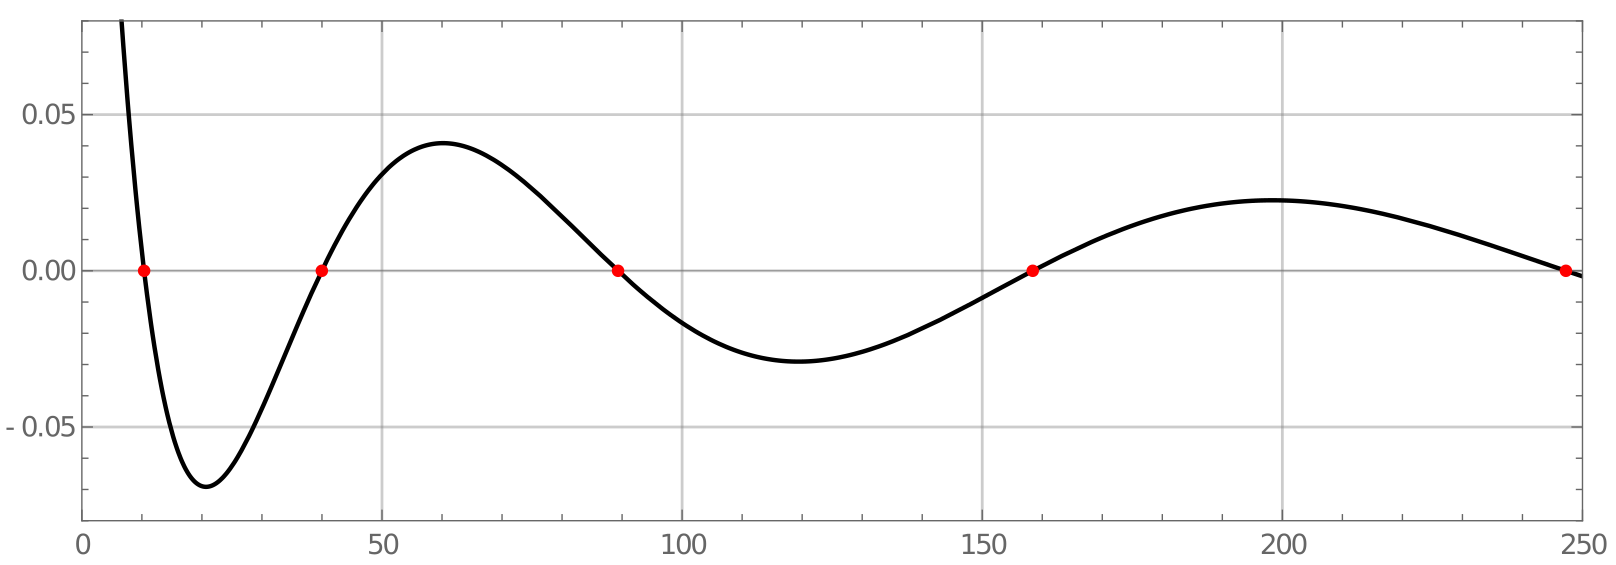
\includegraphics[width=\textwidth]{figures/plot3.png}
	\caption{A comparison of the exact eigenvalues $\alpha$ (the roots of the black curve $\text{det}(\alpha,\beta=1) $), and the approximated eigenvalues (the red points).}
\end{figure}

The approximation breaks down for larger values of $\beta$.  This occurs because the lowest energy eigenvalues obey $\alpha < \beta$.  However, our formula for the asymptotic behavior of the Airy functions required that $\beta - \alpha < 0$.  Hence, the lowest energy eigenvalues are incalculable with the approximation.  However, the higher energy eigenvalues calculated by the approximation still match very well.  Figure 4 is the same as Figure 3, but shows the situation for $\beta = 10$.   

\begin{figure}[ht]
	\centering
	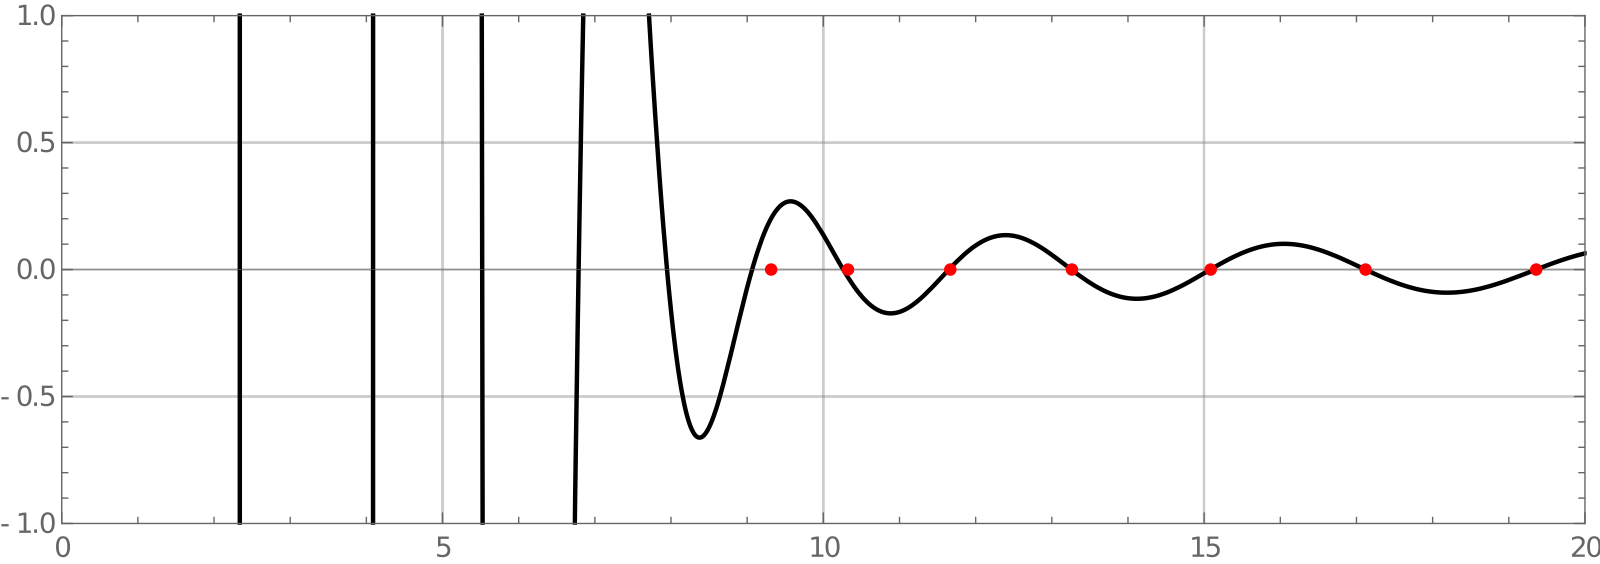
\includegraphics[width=\textwidth]{figures/plot4.png}
	\caption{A comparison of the exact eigenvalues $\alpha$ (the roots of the black curve $\text{det}(\alpha,\beta)$ and the approximated eigenvalues (the red points), for $\beta = 10$.  The first five eigenvalues cannot be calculated with the approximation, but the larger eigenvalues match the exact ones well.}
\end{figure}
\vspace{1cm}






\subsection*{Further Questions}
\noindent (a) For small $L$, the approximation being made is identical to that of large energy.  In both cases, $\alpha \gg \beta$.  

\vspace{1cm}
\noindent (b) For what parameters will the ground state energy equal $FL$?  Note that at $E = FL$, $\alpha = \beta$.  By examining the plot in Figure 1, we see that there are many $(\alpha, \beta)$ that satisfy both $\alpha = \beta$ and $\text{det}(\alpha, \beta) = 0$.  However, only one such point is a ground state.  By inspection that point is near $(3,3).$  The exact location, which can be found numerically, is $(2.666, 2.666)$.  For $\alpha$ and $\beta$ to take on these values, the parameters of the problem will satisfy
\[
	\frac{mFL^3}{\hbar^2} = 9.47.
\] 

\vspace{1cm}
\noindent (c) It is clear just from examining Figure 1 that for all $\beta < 2.666,$ the first ground state will be larger than $E = FL$, or $\alpha = 2.666$.  


\vspace{1cm}

\hfill Contestant: Jacob H. Nie


\medskip








\end{document}
